% Tento soubor nahraďte vlastním souborem s obsahem práce.
%=========================================================================
% Autoři: Michal Bidlo, Bohuslav Křena, Jaroslav Dytrych, Petr Veigend a Adam Herout 2019

% Pro kompilaci po částech (viz projekt.tex), nutno odkomentovat a upravit
%\documentclass[../projekt.tex]{subfiles}
%\begin{document}

%===============================================================================

\newcommand*{\addNewChapter}[2][1]{\addtocounter{chapterCounter}{#1}\chapter{#2}\label{#2}}


\addNewChapter{Úvod}
Komunikácia je neodmysliteľnou súčasťou zdielania a prenosu informácii. V súčasnosti sa na tento účel využíva hlavne výpočtová technológia.

Základ počítačovej komunikácie tvoria dve hlavné zložky: adresovanie a smerovanie. Adresovanie je spôsob vytvárania a priraďovania adries počítačom. 
Adresa je jednoznačný údaj, ktorý presne identifikuje práve jeden adresovateľný prvok. Smerovanie je proces výberu cesty pre prevádzku v sieti medzi viacerými sieťami. \cite{Smerovanie}

Adresa zariadení na úrovni TCP/IP je vo formáte IP adresy (napríklad 95.82.140.207). 
Pre človeka je adresovanie na úrovni počítačov komplikované. Adresovanie počítačov pomocou IP adries nie je nutne dobré riešenie pre užívateľov, pretože sú náročné na zapamätanie.
Z toho dôvodu bol vyvinutý systém, ktorý umožňuje adresovať zariadenia pomocou doménových adries.

\section{Domain name system}
\label{Domain name system}
DNS (angl. domain name system) je systém, ktorého cieľom je poskytnúť mechanizmus na pomenovávanie
zdrojov (zariadení) takým spôsobom, aby tieto mená boli použiteľné v rôznych zariadeniach, sieťach, protokolových rodinách, 
na internete a administratívnych organizáciach. \cite{rfc1035} 

\section{Architektúra DNS}
Základnou úlohou služby DNS je mapovanie doménových adries (tzv. doménových mien) na IP adresy. 
Systém DNS sa skladá z troch hlavných častí - priestoru doménových mien, DNS serverov a resolveru. Priestor doménových mien je databáza, kde sú dané doménové mená uložené. 
Táto databáza je hierarchicky usporiadaná do stromovej štruktúry (pre rýchle vyhladávanie konkrétnych domén). \cite{Matoušek}

\section{DNS resolver}
\label{DNS resolver}
Je to klientský program, ktorý získavá informácie zo systému DNS prostredníctvom dotazovania sa na DNS servery. Tento proces sa nazýva DNS rezolúcia.
Resolver môže mať viac typov konfigurácii. 
Táto práca je zameraná na nárvh a implementáciou tzv. stub resolvera.


\addNewChapter{Návrh programu}

\section{Stub resolver}
\label{Stub resolver}
Stub resolver je typ resolvera, ktorý interaguje s aplikáciou alebo užívateľom a rekurzívnym DNS serverom. Samotný resolver rezolúciu nevykonáva.
V tomto prípade sa rezolúcia realizuje zaslaním dotazu resolvera na rekurzívny DNS server, ktorý odošle odpoveď na dotaz.
Prijatú odpoveď resolver spracuje a získané informácie poskytne aplikácii alebo zobrazí užívateľovi.

\section{Dotazovanie}
\label{Dotazovanie}

Dotazovanie na server prebieha zasielaním správ. Užívateľ alebo aplikácia poskytne údaje resolveru (ako sú dotazovaná adresa, typ dotazu).
Resolver dané údaje vloží do správy, ktorú odošle na DNS server, na čo DNS server odpovie. Komunikácia prebieha štandartne cez protokol UDP. Jeden dotaz zodpovedá jednému UDP datagramu.

\subsection{Formát správy}
\label{Formát správy}

Správa sa skladá z 5 hlavných častí: hlavičky, otázky, odpovednej sekcie, autoritatívnej sekcie a dodatočnej sekcie. 
V hlavičke sú uložené údaje o dotaze, ako ID, typ dotazu, príznaky (dodatočné informácie o správe), kód chyby a čítače záznamov pre jednotlivé sekcie.
Časť otázky sa skladá z dotazovanej adresy rozloženej na časti (tzv. labels), typu dotazu a triedy dotazu (typicky IN pre internet). 

\newpage

\subsubsection{Príznaky}
\begin{itemize}
    \item QR - tento príznak odlišuje dotaz (0) a odpoveď (1)
    \item OPCODE - typ dotazu
    \item AA - ak je nastavený na hodnotu 1, tak odpoveď je autoritatívna (dotazovaný server je autorita pre dotazovanú doménu)
    \item TC - ak je nastavený na hodnotu 1, tak odpoveď je skrátená
    \item RD - ak je nastavený na hodnotu 1, tak je požadovaná rekurzívna rezolúcia
    \item RA - určuje, či je rekurzívna rezolúcia implementovaná v odpovedi
    \item Z - príznak rezervovaný pre budúce použitie (musí byť nulový)
    \item RCODE - kód odpovede
\end{itemize}

Príznaky predstavujú základné informácie o obsahu správy.
Pri zasielaní dotazu sa nastavujú parametre v hlavičke a otázkovej sekcii. Zvyšné sekcie sú určené pre zaznamenanie odpovede. Hodnoty príznakov
QR, AA, TC, RA, Z, RCODE musia byť pri zaslaní dotazu nulové.

\newpage
\section{Objektový nárvh}
\label{Objektový návrh}

\begin{figure}[H]
    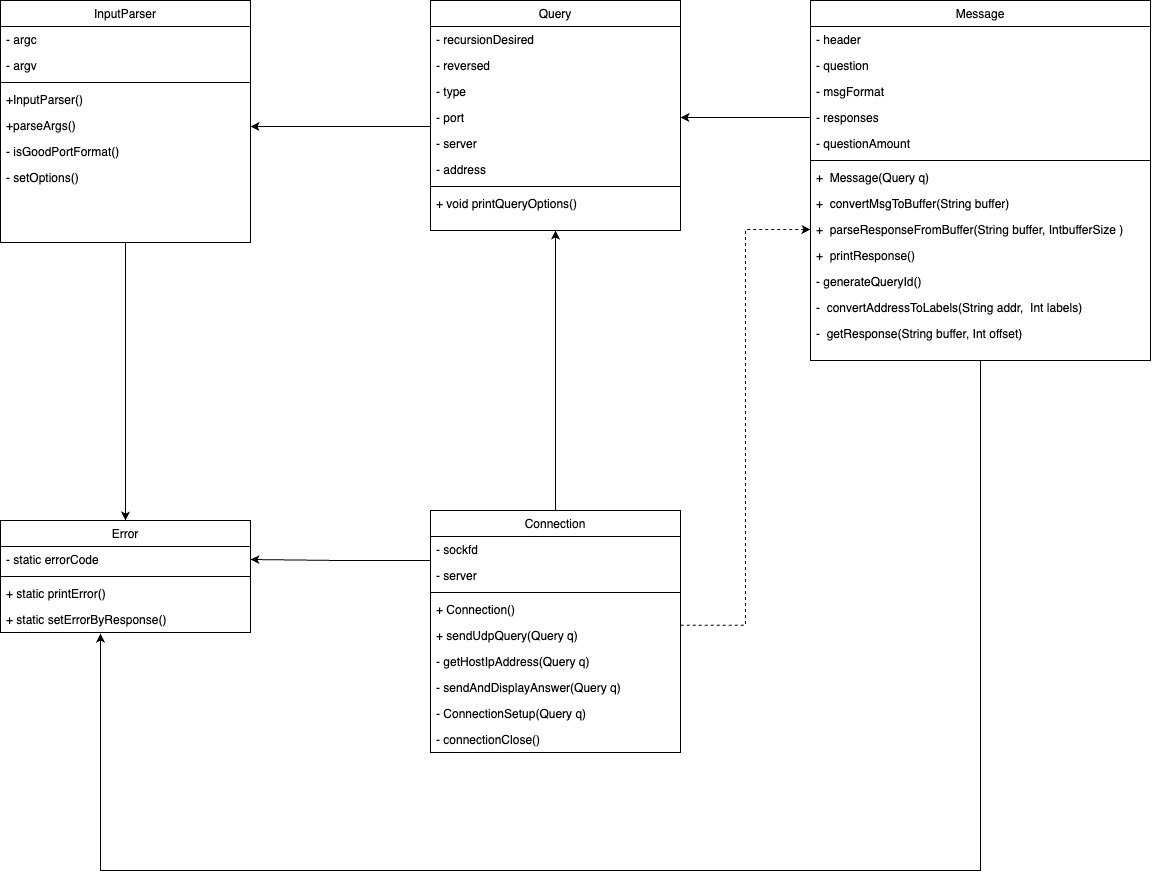
\includegraphics[width=\textwidth]{./template-fig/DNS_resolver.jpg}
    \caption{Class diagram}
    \centering
\end{figure}

Program sa skladá z 5 hlavných tried: InputParser, Query, Message, Connection a Error. Prvé 4 triedy spravujú správy a trieda Error spracováva chybové stavy, chybové hlásenia a návratovú hodnotu programu.

Trieda InputParser má za úlohu spracovať argumenty zadané používateľom a vytvoriť dotaz. Dotaz reprezentuje trieda Query.
Spracovanie dotazu, jeho zaslanie a prijatie odpovede má za úlohu trieda Connection. Trieda Message slúži na vytvorenie správy z dotazu a jej konverziu medzi 
formátom, ktorý sa odosiela po sieti a formátom, ktorý spracováva aplikácia.


\addNewChapter{Popis programu}

\section{Vstup}
\label{Vstup}

Program príjma vstupy z príkazovej riadky pri spustení. 
\begin{verbatim}
    ./dns [-r] [-x] [-6] -s server [-p port] address
\end{verbatim}
    
Popis prepínačov:
\begin{itemize}
    \item -r nastaví príznak pre rekurzívny dotaz
    \item -x nastaví príznak pre reverzný dotaz 
    \item -6 nastaví príznak pre dotazovanie sa na adresy IPv6 
    \item -s povinný prepínač; za ním nasleduje adresa serveru
    \item server je adresa serveru, na ktorý budeme posielať dotaz
    \item -p nepovinný prepínač; nastaví číslo portu
    \item address je adresa, na ktorú sa budeme dotazovať
\end{itemize} 

V prípade použitia nedefinovaného prepínača program vypíše chybové hlásenie a program skončí. 
V prípade viacerých zadaných prepínačov -s program použije poslednú zadanú adresu serveru. To isté platí pre zadávanie adries.
Ak je pri zadávaní portu zadaný port v neplatnom formáte, program použije štandartný port pre DNS (port číslo 53).

\section{Výstup}
\label{Výstup}
Výstup z programu je vo formáte
\begin{verbatim}
Authoritative: No, Recursive: Yes, Truncated: No
Question section (1)
  www.fit.vut.cz., A, IN
Answer section (1)
  www.fit.vut.cz., A, IN, 14400, 147.229.9.26
Authority section (0)
Additional section (0)
\end{verbatim}

Kde \textsc{Authoritative: No} značí, že dotazovaný server nie je autorita pre danú doménu, \textsc{Recursive: Yes} značí, či bol odpoveď nájdená rekurzívne,
a \textsc{Truncated: No} značí, že odpoveď nebola skrátená. V prípade skrátenej odpovede vypíše program na výstup túto informáciu sekciu otázky. Zvyšné sekcie program nevypíše.

\noindent Štandartný formát odpovede: <dotazovaná doména>, <typ záznamu>, <trieda dotazu>, <ttl>, <dáta odpovede>. 

Návratové hodnoty:
\begin{itemize}
    \item 0 : úspech
    \item 1 - 5 : kód chyby získanej od serveru
    \item 6 : zlyhanie spojenia
    \item 7 : zlé vstupné parametre
    \item 99 : interná chyba programu
\end{itemize}


\section{Príklad spustenia}
\label{Príklad spustenia}

Príklad rekurzívneho spustenia:

\begin{verbatim}
    ./dns -r -s dns.google.com www.fit.vut.cz  
\end{verbatim}

\noindent Výstup:

\begin{verbatim}
Authoritative: No, Recursive: Yes, Truncated: No
Question section (1)
  www.fit.vut.cz., A, IN
Answer section (1)
  www.fit.vut.cz., A, IN, 12283, 147.229.9.26
Authority section (0)
Additional section (0)
\end{verbatim}

Príklad nerekurzívneho spustenia

\begin{verbatim}
    ./dns -s kazi.fit.vutbr.cz www.vut.fit.cz
\end{verbatim}

\noindent Výstup:
\begin{verbatim}
Authoritative: No, Recursive: No, Truncated: No
    Question section (1)
      www.vut.fit.cz., A, IN
    Answer section (0)
    Authority section (4)
      cz., NS, IN, 172800, b.ns.nic.cz.
      cz., NS, IN, 172800, c.ns.nic.cz.
      cz., NS, IN, 172800, d.ns.nic.cz.
      cz., NS, IN, 172800, a.ns.nic.cz.
    Additional section (8)
      d.ns.nic.cz., A, IN, 172800, 193.29.206.1
      c.ns.nic.cz., A, IN, 172800, 194.0.14.1
      b.ns.nic.cz., A, IN, 172800, 194.0.13.1
      a.ns.nic.cz., A, IN, 172800, 194.0.12.1
      d.ns.nic.cz., AAAA, IN, 172800, 2001:678:1:0:0:0:0:1
      c.ns.nic.cz., AAAA, IN, 172800, 2001:678:11:0:0:0:0:1
      b.ns.nic.cz., AAAA, IN, 172800, 2001:678:10:0:0:0:0:1
      a.ns.nic.cz., AAAA, IN, 172800, 2001:678:f:0:0:0:0:1
\end{verbatim}

\section{Zaujímavé časti kódu}
\label{Zaujímavé časti kódu}

\subsection{Vytváranie spojenia}
\label{Vytváranie spojenia}
Pre vytovernie spojenia je treba získať najprv adresu zo serveru. Získavanie adresy serveru je realizovná prostredníctvom vstavanej funkcie 
\verb|gethostbyname()|.


\subsubsection{Použitie funckie gethostbyname():}
\begin{verbatim}
// check if host was found
hostInfo = gethostbyname(server);
if (hostInfo == NULL)
{
    Error::printError(CONNECTION_FAILED, "Host IP address not found.\n");
    return false;
}

// get ip address
struct in_addr **addressList = (struct in_addr **)hostInfo->h_addr_list;
if (addressList == NULL)
{
    Error::printError(CONNECTION_FAILED, "Host IP address not found.\n");
    return false;
}
\end{verbatim}

\newpage
\noindent Získanie adresy z vráteného listu adries:
\begin{verbatim}
for (size_t i = 0; addressList[i] != NULL; i++)
{
    char *ipAddr = inet_ntoa(*addressList[i]);
    if (inet_pton(AF_INET, ipAddr, &dst->s_addr) < 1)
    {
        // if there is no more ip address in list, get error
        if (addressList[i + 1] == NULL)
        {
            Error::printError(CONNECTION_FAILED, "Host IP address 
            not found.\n");
            return false;
        }
    }
    // found
    else
    {
        break;
    }
}
\end{verbatim}

\noindent Obe časti kódu su prevzaté zo stránky GeeksForGeeks \cite{gethostbyname}.

Po získaní adresy môžeme prejsť k zahájeniu sponia. Samotné spojenie je realizované pomocou UDP schránok:

\subsubsection{Príprava spojenia}
\begin{verbatim}
    this->sockfd = socket(AF_INET, SOCK_DGRAM, 0);
    if (sockfd < 0)
    {
        Error::printError(CONNECTION_FAILED, "socket() failed\n");
        return false;
    }

    // setup server address
    memset(&this->server, 0, sizeof(sockaddr_in));

    struct in_addr serverAddr;
    if (!getHostIPaddress(query.getServer().c_str(), &serverAddr))
    {
        return false;
    }

    this->server.sin_addr = serverAddr;
    this->server.sin_port = htons(query.getPort());
    this->server.sin_family = AF_INET;
\end{verbatim}

\subsubsection{Odoslanie query}
\begin{verbatim}
    if (connect(this->sockfd, (struct sockaddr *)(&this->server), 
    sizeof(this->server)) < 0)
    {
        Error::printError(CONNECTION_FAILED, "connect() failed\n");
        return;
    }
    
    ...

    int bytesTx = send(this->sockfd, (const char *)buffer, 
    bufferLength, 0);
    if (bytesTx < 0)
    {
        Error::printError(CONNECTION_FAILED, "send() failed\n");
        return;
    }
\end{verbatim}


\subsubsection{Príjmanie odpovede}

\begin{verbatim}
    char recvBuffer[UDP_DATAGRAM_LIMIT] = {0};
    int bytesRx = recv(this->sockfd, (char *)recvBuffer, 
    UDP_DATAGRAM_LIMIT, 0);
    if (bytesRx < 0)
    {
        Error::printError(CONNECTION_FAILED, "recv() failed\n");
        return;
    }
\end{verbatim}

Zdroj: \cite{UDPSockets}

\subsubsection{Timeout}
Pre prípad, že server nepošle odppoveď, alebo služba na danom serveri nebeží, je v tomto resolveri implementovaný timeout.\cite{timeout}

\begin{verbatim}
    struct timeval timeout;
    timeout.tv_sec = 2;
    timeout.tv_usec = 0;
    setsockopt(this->sockfd, SOL_SOCKET, SO_RCVTIMEO, 
    (const char *)&timeout, sizeof(timeout));
\end{verbatim}

\section{Kompatibilita}
\label{Kompatibilita}
Program bol vyvíjaný pomocou jazyka C++. Pre preklad bol použitý nástroj GNU Make 3.81. Preklad bol prekladaný pomocou štandardu c++17.
Program Kompatibilný s operačnými systémami typu UNIX. 

\addNewChapter{Testovanie}

\section{Spôsoby testovania}
\label{Spôsoby testovania}
Program bol testovaný dvomi spôsobmi: neformálnym testovaním programátorom a formálnym testovaním pomocou automatizovaných testov.
Neformálne boli testované hlavne nevalidné vstupy a formát výstupu. 
Pomocou automatických testov boli testované prípady a hodnoty výstupov. Spustenie automatických testov sa realizuje pomocou priloženého Makefile súboru príkazom \verb|make test|.

\section{Použité nástroje}
\label{Použité nástroje}
Ako nástroje na automatické testy boli použité python3 verzia Python 3.10.0. Testovanie bolo vykonávané na princípe 
porovnávania výstupov s programom DiG verzie 9.10.6.

\section{Testovacie prostredie}
\label{Testovacaie prostrede}
Program bol vyvíjanú v prostredí macos Ventura 13.6 s ARM procesorom. Testovanie prebiehalo lokálne, ale aj 
na serveri merlin (\url{https://merlin.fit.vutbr.cz/}) a na serveri eva (\url{https://eva.fit.vutbr.cz/}).




